%Please use LuaLaTeX or XeLaTeX
\documentclass[11pt,aspectratio=169]{beamer}

\usepackage[ngerman]{babel}
\usepackage{ragged2e}

\definecolor{ethblue}{RGB}{32, 91, 174}
\definecolor{mygrey}{RGB}{175, 175, 175}

\hypersetup{
  colorlinks=true,
  urlcolor=ethblue,
  linkcolor=ethblue,
  citecolor=ethblue
}

\title{Theoretische Informatik}
% \date[ABC 2021]{24. Sep 2026}
\date[]{22. Okt 2026}
\author{Olivér Kovács}
% \institute{Organizational Unit\\can spread over 2 lines}

\usetheme{eth}

\colorlet{titlefgcolor}{ETHBlue}
\colorlet{accentcolor}{ETHRed}

\begin{document}

%\def\titlefigure{elements/title-page-image}		% Default image
%\def\titlefigure{elements/title-page-image-43}	% Use this for 4:3 presentations

\titleframe

% \tocframe

% \section{Layout}

\begin{frame}{Midterm}
    Altklausuren: \href{https://exams.vis.ethz.ch/}{https://exams.vis.ethz.ch/}

    \vspace{1em}

    Stoff hat sich geändert:
    \begin{itemize}
    \item
        Kolmogorovkomplexität, Satz 3.1 nicht relevant.
    \item
        Relevant bis einschliesslich
        \begin{itemize}
            \item
                Vorlesung am 03. Novemeber,
            \item
                Blatt 6,
            \item
                Quiz 7.
        \end{itemize}
    \item Manches davon war früher nicht auf den Midterms!
    \end{itemize}
\end{frame}

\begin{frame}{Nebenbemerkung: Minimalität von DEAs}
    \begin{itemize}
    \item
        Zwei Zustände \(p, q \in Q\) in einem DEA können nicht
        zusammengefasst werden gdw ein Wort \(w\) existiert,
        so dass gilt
        \[
            \hat\delta(p, w) \in F \iff \hat\delta(q, w) \not\in F.
        \]
    \item
        Ein DEA ist minimal gdw für alle Zustände paarweise gilt,
        dass sie nicht zusammengefasst werden können, und
        \textbf{jeder Zustand erreichbar} ist.
        \vspace{1em}
    \item
        Bitte einfach Beweis schreiben wie in der Vorlesung
        hergezeigt!
    \end{itemize}
\end{frame}

\begin{frame}{Bemerkungen zur Serie}
    \begin{itemize}
    \item
        In unserem Formalismus sind in NEAs \textbf{keine}
        \(\lambda\)-Transitionen erlaubt!
        \vspace{1em}
    \item
        Startzustand und akzeptierenden Zustände nicht vergessen.
        \begin{itemize}
            \item Insbesondere \(\lambda\) beachten!
        \end{itemize}
        \vspace{1em}
    \item
        Bei Minimalitätsbeweis:
        \begin{itemize}
            \item Bitte Tabelle wie in der Vorlesung.
            \item Lemma 3.3 erwähnen.
            \item Landen die Wörter tatsächlich in verschiedenen Zustände?
            \item Man darf \(\lambda\) als Suffix wählen.
        \end{itemize}
    \end{itemize}
\end{frame}

\begin{frame}{Quiz}
    Gibt es Fragen zum Quiz?
\end{frame}

\begin{frame}{Turingmaschine}

\textbf{Definition 4.1.}
Eine \textit{Turingmaschine (TM)} ist ein 7-Tupel
\(M = (Q, \Sigma, \Gamma, \delta, q_0, q_{\text{accept}}, q_{\text{reject}})\).
Dabei ist

\begin{itemize}
    \item \(Q\) die \textit{Zustandsmenge} von \(M\),
    \item \(\Sigma\) das \textit{Eingabealphabet},
    \item \(\Gamma\) das \textit{Arbeitsalphabet},
    \item \(\delta : (Q - \{q_{\text{accept}}, q_{\text{reject}}\}) \times \Gamma
        \to Q \times \Gamma \times \{L, R, N\}\) die \textit{Übergangsfunktion},
    \item \(q_0 \in Q\) der \textit{Anfangszustand},
    \item \(q_{\text{accept}} \in Q\) der \textit{akzeptierende Zustand},
    \item \(q_{\text{reject}} \in Q\) der \textit{verwerfende Zustand}.
\end{itemize}

\end{frame}

\begin{frame}{Rekursiv aufzählbar}
    \textbf{Definition 4.1.}
    [...] Eine Sprache \(L \subseteq \Sigma^*\) heist
    \textit{rekursiv aufzählbar} falls eine TM \(M\) existiert,
    so dass \(L = L(M)\).

    \vspace{1em}

    \[
        \mathcal L_{\text{RE}} = \{L(M) \mid M \text{ ist eine TM}\}
    \]

    ist die \textit{Klasse aller rekursiv aufzählbaren Sprachen}.

\end{frame}

\begin{frame}{Mehrband-Turingmaschine (MTM)}

\textbf{Abbildung 4.7.}
Eine \(k\)\textit{-Band-Turingmaschine} besteht aus
\begin{itemize}
\item
    einer endlichen Kontrolle,
\item
    einem endlichen Eingabeband mit einem Lesekopf,
\item
    \(k\) Arbeitsbänder, jeweils mit einem Lese-/Schreibkopf.
\end{itemize}

\vspace{1em}

Insbesondere ist eine 1-Band-TM nicht das gleiche
wie eine TM!

\end{frame}

\begin{frame}{Äquivalenz}

    \textbf{Lemma 4.1}:
    Für jede TM existiert eine äquivalente 1-Band-TM.

    \vspace{1em}

    \textbf{Lemma 4.2}:
    Für jede MTM existiert eine äquivalente TM.

    \vspace{1em}

    Beweis?

\end{frame}

\begin{frame}{Nebenbemerkung}
    \begin{center}
        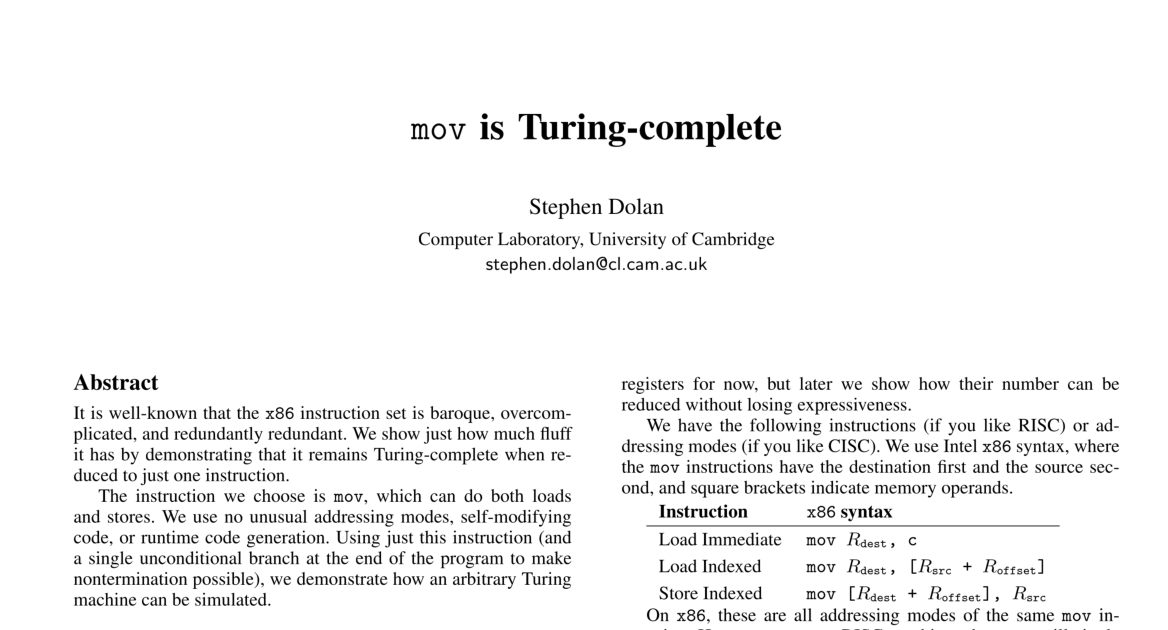
\includegraphics[width=28em]{img/mov}
    \end{center}
\end{frame}

\begin{frame}{Church'sche These}
    
    \justifying

    Die Turingmaschinen sind die Formalisierung des Begriffes „Algorithmus“,
    d.h., die Klasse der rekursiven Sprachen (der entscheidbaren Entscheidungs-
    probleme) stimmt mit der Klasse der algorithmisch (automatisch) erkennbaren
    Sprachen überein.

\end{frame}

\begin{frame}{Nichtdeterminismus}
    
    \justifying

    Eine \textit{nichtdeterministische Turingmaschine (NTM)} ist ein 7-Tupel \\
    \(M = (Q, \Sigma, \Gamma, \delta, q_0, q_{\text{accept}}, q_{\text{reject}})\).
    Dabei

    \begin{itemize}
        \item sind \(Q, \Sigma, \Gamma, q_0, q_{\text{accept}}, q_{\text{reject}}\) gleich wie bei einer TM,
        \item ist \(\delta \colon (Q - \{q_{\text{accept}}, q_{\text{reject}}\}) \times \Gamma \to
            \mathcal P(Q \times \Gamma \times \{\text{L}, \text{R}, \text{N}\})\) die \textit{Übergangsfunktion}.
    \end{itemize}

\end{frame}

\begin{frame}{Äquivalenz}
    
    \textbf{Satz 4.2.} Für jede NTM existiert eine äquivalente TM.

    \vspace{1em}

    Beweis?
\end{frame}

\begin{frame}{Kodierung}

    Wir können Turingmaschinen als Wörter über \(\Sigma_{\text{bool}}\) darstellen. (Wie?)

    \vspace{1em}

    \textbf{Definition 4.5.}
    \(\text{Kod}(M)\) ist die \textit{Kodierung} der TM \(M\).
    Wir definieren

    \[
        \text{KodTM} = \{\text{Kod}(M) \mid M \text{ ist eine TM}\}.    
    \]

\end{frame}

\begin{frame}{Abzählbarkeit}

    \textbf{Definition 5.1.}
    Seine \(A, B\) zwei Mengen.
    Wir sagen, dass
    \begin{enumerate}
        \item \(|A| \le |B|\) falls eine injektive Funktion \(f : A \to B\) existiert,
        \item \(|A| = |B|\) falls \(|A| \le |B|\) und \(|B| \le |A|\) gilt,
        \item \(|A| < |B|\) falls \(|A| \le |B|\) und nicht \(|B| \le |A|\) gilt.
    \end{enumerate}

    \vspace{1em}

    \textbf{Definition 5.2.}
    Eine Menge \(A\) heisst \textit{abzählbar} gdw \(A\) endlich ist oder \(|A| = |\mathbb N|\).

\end{frame}

\begin{frame}{Abzählbarkeit (2)}

    \textbf{Lemma 5.1.}
    Sei \(\Sigma\) ein beliebiges Alphabet.
    Dann ist \(\Sigma^*\) abzählbar.

    \vspace{1em}

    \textbf{Satz 5.1.}
    Die Menge \(\text{KodTM}\) der Turingmaschinenkodierung ist abzählbar.

    \vspace{1em}

    \textbf{Lemma 5.2.}
    Die Menge \((\mathbb N - \{0\}) \times (\mathbb N - \{0\})\) ist abzählbar.

    \vspace{1em}

    \textbf{Satz 5.2.}
    \(\mathbb Q^+\) ist abzählbar.

    \vspace{1em}

    \textbf{Satz 5.3.}
    \([0, 1]\) ist nicht abzählbar.

    \vspace{1em}

    \textbf{Satz 5.4.}
    \(\mathcal P((\Sigma_{\text{bool}})^*)\) ist nicht abzählbar.

    \vspace{1em}

    \textbf{Korollar 5.1.}
    \(|\text{KodTM}| < |\mathcal P((\Sigma_{\text{bool}})^*)|\) und somit existieren unendlich
    viele nicht rekursiv aufzählbare Sprachen.

\end{frame}

\begin{frame}{Diagonalsprache}

    \justifying

    \textbf{Definition.}
    Seien \(w_1, w_2, w_3, \ldots\) die Wörter über \(\Sigma_{\text{bool}}\) in kanonischer Ordnung
    und \(M_1, M_2, M_3, \ldots\) die Folge aller Turingmaschinen. Wir definieren die
    \textit{Diagonalsprache} \(L_{\text{diag}}\) als

    \[
        L_{\text{diag}} =
        \{ w \in (\Sigma_{\text{bool}})^* \mid w = w_i \text{ und } M_i \text{ akzeptiert } w_i \text{ nicht} \}.
    \]

    \vspace{1em}

    \textbf{Satz 5.5.} \(L_{\text{diag}} \not\in \mathcal L_{\text{RE}}\).
\end{frame}

% \setbeamertemplate{footline}{}

\begin{frame}{Aufgaben}
    \begin{enumerate}
        \justifying
        \item 
            \textbf{Aufgabe 1.}
            Worked Example 1.
        \item
            \textbf{Aufgabe 2.}
            Beschreibe informell eine NTM, welche die Sprache
            \[
                L_{\text{composite}} = \{ w = 0^n \mid n \in \mathbb N \text{ ist nicht prim}\}
            \]
            akzeptiert.
        \item
            \textbf{Aufgabe 3.}
            Wir betrachten die Sprache
            \[
                L_{\lambda + 1} = \{\text{Kod}(M) \mid \text{TM } M \text{ akzeptiert } \lambda \text{ und mindestens ein weiteres Wort}\}.
            \]
            Zeige, dass \(L_{\lambda + 1} \in \mathcal L_{\text{RE}}\).
    \end{enumerate}
\end{frame}

\end{document}
